% Seminar Information Retrieval Philipp Schalcher
% Betreuer: Ruxandra Domenig
% Thema: Evaluierung der Retrieval-Leistung einer Search Engine am Beispiel einer privaten MP3-Sammlung

\documentclass[12pt,a4paper,ngerman]{report}
\setlength{\parindent}{0pt}
\usepackage[ngerman]{babel}
\usepackage[utf8]{inputenc}
\usepackage{a4wide}
\usepackage{graphicx}
\usepackage{url}
\usepackage[final]{listings}
\usepackage{color}
\usepackage{amsmath}
\author{Philipp Schalcher}
\title{Evaluierung der Retrieval-Leistung einer Search Engine am Beispiel einer privaten MP3-Sammlung}
\date{\today}

\begin{document}
%\maketitle
\begin{titlepage}
\begin{center}

\includegraphics[width=0.25\textwidth]{img/zhaw.png}\\[0.5cm]
\textsc{\Large Zürcher Hochschule für Angewandte Wissenschaften}\\[1.0cm]
\textsc{\Large Seminar Information Retrieval}\\[1.5cm]

% Title
\hrulefill \\[0.5cm]
{\huge \bfseries Evaluierung der Retrieval-Leistung einer Search Engine am Beispiel einer privaten MP3-Sammlung}\\[0.4cm]
\hrulefill \\[0.5cm]
%Author und Betreuer
\begin{minipage}{0.4\textwidth}
\begin{flushleft}
\emph{Author:}\\
Philipp \textsc{Schalcher}
\end{flushleft}
\end{minipage}
\begin{minipage}{0.4\textwidth}
\begin{flushright}
\emph{Betreuer:}\\
Ruxandra \textsc{Domenig}
\end{flushright}
\end{minipage}

\vfill

%Datum
{\large \today}

\end{center}
\end{titlepage}
\chapter*{Danksagung}
\tableofcontents
\begin{abstract}

\end{abstract}
\chapter{Einleitung}
In der heutigen Zeit wird der Mensch von einer Fülle an Informationen überflutet. Würde er nicht gewisse Eindrücke selber filtern, könnte das zu einem Kollaps führen. Der Mensch hat das Glück, solche Dinge von der Natur eingebaut zu haben. Im Gegensatz zum Menschen besitzen Informationssysteme keine integrierten Filter. Das beste Beispiel hierfür ist Google. Es gibt eine riesige Menge an Daten, die der Suchmaschine ihr Wissen verleiht.
\\
\\
Lucene ist eine Bibliothek, welche in verschiedene Projekte eingebaut werden kann, um so eine mächtige Suchmaschine auf Basis von Indexen zu bekommen. Lucene enthält alle relevanten Funktionen, die benötigt werden, um Informationen zu durchsuchen. Hier liegt die Herausforderung, eine Suchmaschine für ID3-Tags von MP3-Dateien zu bauen, da Lucene hauptsächlich für Textdateien (PDF,TXT,DOCX,eBooks,usw.) genutzt wird. Für MP3-Dateien stehen andere Probleme an (Wie extrahiere ich die ID3-Tags aus einer MP3-Datei). 
\\
\\
Diese Arbeit soll die Information Retrieval Leistung der Suchengine Lucene analysieren. Darin enthalten sind eine Programmierung einer kleinen Suchmaschine, die MP3-Dateien innerhalb eines Ordners indexiert und danach durchsucht. Dabei beschränke ich mich in der praktischen Arbeit auf das indexieren der ID3-Tags. Diese Arbeit soll nicht als Anleitung zur Erstellung einer Suchmaschine dienen!
\\
\\
Da Lucene natürlich auch den Inhalt einer Datei analysiert, muss diese Arbeit ein bisschen angepasst werden. Da MP3-Dateien keinen Text als Inhalt haben, möchte ich daher nur theoretisch aufzeigen, wie anhand von Teilen eines Liedes das entsprechende Lied gesucht werden kann. Dies zu programmieren sprengt den Rahmen der Arbeit, somit werde ich am Beispiel von Shazam nur eine theoretische Lösung aufzeigen.
\chapter{Hauptteil}
\section*{Lucene}
Was ist Lucene? Dies ist die erste Frage, die ich mir zu Beginn der Arbeit gestellt habe. Da mir das Produkt gänzlich unbekannt war, galt es zuerst Informationen zu sammeln.\\
\\
Apache Lucene eine Suchengine, die sich auf Text und eine hohe Performance spezialisiert hat. Dabei ist die Engine mittlerweile in verschiedene Sprachen übersetzt worden. Der Apache Lucene Core ist der Hauptteil der Software und ist in Java geschrieben. Das beste an Lucene ist wohl, dass es gratis zur Verfügung steht. Somit kann jeder Entwickler eine mächtige Suchmaschine in seine Programme einbauen. \\
\\
Bei einer Suchmaschine liegen die Stärken im Resultat welches geliefert wird. Lucene bietet auch hier wieder einige Funktionen, die das Endergebnis schnell und korrekt ergeben sollen. Dazu gehören:
\begin{itemize}
	\item Ranked Searching - Die besten Resultate werden als Erste zurückgegeben.
	\item Verschiedene Query-Typen
	\item Feldsuche (Hier Titel, Album, Künstler, Jahr).
	\item Mehrfache Indexe durchsuchen mit zusammengefasstem Ergebnis.
	\item Schnell
	\item Speichereffizient
	\item Tippfehler-tolerant
\end{itemize}
Mit diesen und weiteren Gimmicks wird Lucene auf der Webseite \url{lucene.apache.org/core/} angepriesen. Für meine Arbeit habe ich die Bibliothek in der Version 3.6.2 verwendet, da meine Quelle ebenfalls mit einer 3er-Version gearbeitet hat.
\section*{Information Retrieval}
\begin{quote}
The IR Problem: The primary goal of an IR system is to retrieve all the documents that are relevant to a user query while retrieving as few non-relevant documents as possible. - Buch: Modern Information Retrieval
\end{quote}
Dieses Zitat bezeichnet sehr gut um was es bei Information Retrieval geht. Die Menschheit speichert seit 5000 Jahren Informationen in verschiedenen Systemen, um danach über Indexe oder andere Suchmechanismen an wichtige Informationen zu kommen. Im einfachsten Fall möchte ein User nach einer Suche einen Link zu einer Webseite von einer Organisation, Firma oder sonstigen Quelle. Information Retrieval alleine dreht sich nicht nur um Suchmaschinen. Die Definition aus dem Buch Modern Information Retrieval lautet wie folgt:
\begin{quote}
Information retrieval deals with the representation, storage, organization of, and access to information items such as documents, Web pages, online catalogs, structured and semi-structured records, multimedia objects. The representation and organization of the information items should be such as to provide the users with easy access to information of their interest. - Buch: Modern Information Retrieval
\end{quote}
Zu Beginn war Information Retrieval nur eine Kategorie, die für Bibliothekare und Informationsexperten interessant war. Dieser Umstand änderte sich aber schlagartig, als das Internet aufkam. Informationen waren nun zugänglich und konnten von fast jedem Menschen abgerufen werden. Mit dem Internet wurde es wichtiger, gute Ergebnisse beim Suchen nach Informationen zu bekommen. Information Retrieval hatte die breite Masse erreicht.\\
\\
Ein Grundproblem bei IR-Systemen ist, welche Informationen für die gewünschte Suche überhaupt relevant sind. Wie soll die Software entscheiden, welche Informationen am besten auf die Anforderungen des Benutzers zutreffen? Dabei gibt es verschiedene Möglichkeiten. Ein Beispiel ist das sogenannte Ranking. Dabei wird einem Dokument, welches häufiger erscheint, ein höheres Ranking gegeben. Somit weiss die Suchmaschine, dass es wahrscheinlicher ist, dass in diesem Dokument gesuchte Informationen zu finden sind, die mit den Anforderungen übereinstimmen.\\
Eine weitere Möglichkeit besteht in der örtlichen Ablage von Informationen. So können die \textquotedblleft am nächsten liegenden\textquotedblright Informationen auch die richtigen sein. Suche ich zum Beispiel in Google nach einem Detailhändler, möchte ich natürlich die Händler im Ergebnis erhalten, die am nächsten zu mir liegen.\\
Als Drittes ist die Grösse eines Dokumentes ebenfalls eine Variable. So können kleine Dokumente bevorzugt werden, da sie schnell heruntergeladen und veranschaulicht werden können.
\newpage
Information Retrieval Systeme müssen komplexe Anforderungen erfüllen. Mit den oben genannten drei Beispielen für Ergebnissen, folgt der Schluss, dass IR-Systeme nie die eine perfekte Lösung anbieten können. Die Anfragen sind zu komplex um alle möglichen Varianten in eine Suchmaschine zu integrieren.\\
\\
Lucene ist genau solch ein IR-System. Dieses System soll nun analysiert werden. Darunter fällt die Analyse der verschiedenen Analyzer. Konkret handelt es sich um den Standard Analyzer, den Whitespace Analyzer, den Stop Analyzer und den Simple Analyzer. Hier möchte ich mich darauf konzentrieren, wie genau die Informationen in den Index gespeichert werden. Ein ebenfalls wichtiger Faktor ist die Zeit. Einerseits die Dauer der Indexerstellung und danach die Dauer der Suche mit den verschiedenen Einstellungen. Als Letztes möchte ich mich um die Analyse des Ergebnisses kümmern, wobei ich eine Testmenge an MP3 benutze um damit die tatsächlichen Suchergebnisse mit der erwarteten Menge zu vergleichen.
\section*{Lucene Search Engine}
Das entwickelte Programm hat den Namen \textquotedblleft Lucene Search Engine\textquotedblright und wurde in Java entwickelt. Im Programm kann unter dem Punkt \textquotedblleft Pfad\textquotedblright der Ablageort der MP3-Dateien angegeben werden. Mit dem Button Index wird dann in diesem Pfad ein Ordner Index erstellt, in welchem der Lucene-Index erstellt wird. Dabei durchsucht das Programm alle MP3-Dateien im angegeben Pfad, auch in Unterordnern. Aus diesen Dateien werden dann die Informationen Titel, Album, Künstler, Jahr, Pfad und Dateiname extrahiert und in den Index geschrieben. Gesucht wird dann in den Feldern Titel, Album, Künstler, Jahr und Dateiname. Als Ergebnis wird der Pfad zur entsprechenden Dateien ausgegeben.
\newpage
\subsection*{Das GUI}
In diesem Abschnitt möchte ich ganz kurz die grafische Benutzeroberfläche erläutern. Ich gehe nicht weiter auf die Programmierung ein, da dies nur ein kleiner, eher unwichtiger Teil der Search Engine ist.
\begin{figure}[h!]
\centering
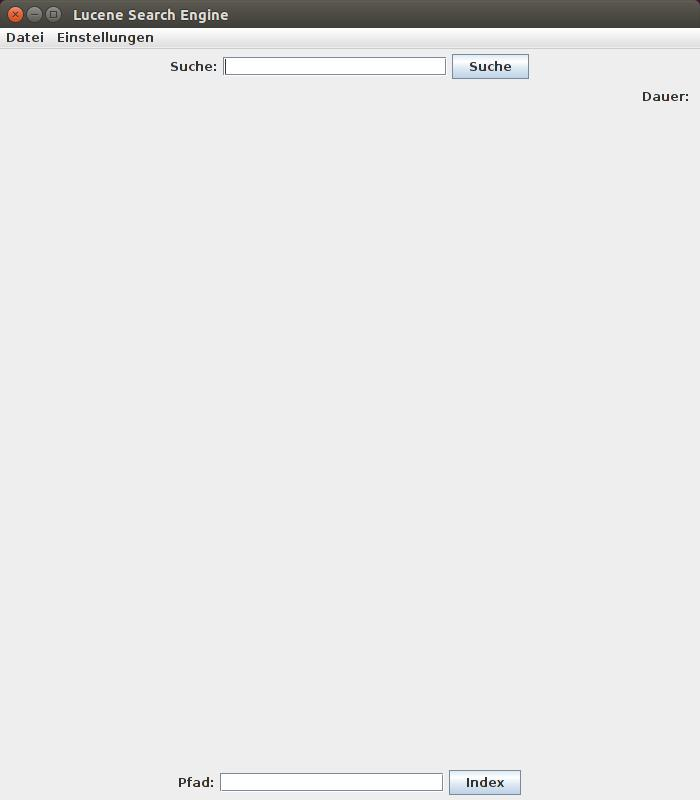
\includegraphics[width=10cm]{img/Lucene_Search_Engine_1.jpg}
\caption{GUI des Programmes\protect\footnotemark}
\end{figure}
\footnotetext{Quelle: Screenshot}
Zuerst betrachten wir die Menüleiste. Unter dem Punkt Datei ist nicht weiteres zu finden als ein Punkt \textquotedblleft Schliessen\textquotedblright der das Programm beendet. Interessanter ist da der Punkt Einstellungen. Öffnet man diesen, erhält man eine Auswahl der 4 erwähnten Analyzer. Je nach Auswahl wird der Index auf andere Weise erstellt und die Suche durchgeführt. Es kann jeweils nur ein Analyzer ausgewählt werden. Falls man ihn ändert sollte man auch den Index neu erstellen.
\subsubsection*{Indexieren}
Am unteren Rand der Applikation befindet sich das Feld Pfad. Dort wird der Pfad zu den abgelegten Dateien eingefügt. Dies funktioniert für Linux wie für Windows und Mac. Sobald dies erledigt wurde, kann mit dem Knopf die Indexierung gestartet werden. Als Analyzer wird die Auswahl aus den Einstellungen genommen. Der Index wird im gleichen Pfad erstellt und in einem Unterordner mit dem Namen \textquotedblleft Index\textquotedblright abgelegt. Dies geschieht automatisch und kann nicht geändert werden. Sobald die Indexierung beendet ist, wird auf der rechten Seite die Dauer in Millisekunden angezeigt. Je mehr MP3-Dateien indexiert werden müssen, desto länger dauert der Vorgang.
\begin{figure}[h!]
\centering

\includegraphics[width=10cm]{img/Pfadangabe.png}
\caption{Beispiel eines angegebenen Pfades in Ubuntu\protect\footnotemark}
\end{figure}
\footnotetext{Quelle: Screenshot}
Nach der Indexierung ist die Suchmaschine bereit und kann verwendet werden. Das praktische an dieser Lösung liegt darin, dass die MP3-Dateien zum Beispiel auch auf einem externen Speichermedium liegen können und der Index auf diesem Medium erstellt werden kann (gilt natürlich nicht für CD/DVDs). So kann theoretisch für jeden Ablageort eine eigener Index erstellt werden. Genaueres zur Indexierung und wie sie gelöst wurde ist im Abschnit \textquotedblleft Der Indexer\textquotedblright zu lesen.
\subsubsection*{Suchen}
Als Erstes muss gesagt werden, dass für die Suche das Pfadfeld weiterhin den Eintrag enthalten muss. Dies ist wichtig, da sonst die Engine nicht weiss, wo sich der Index befindet. Am oberen Rand befindet sich das Suchfeld. Der Benutzer kann hier seine Suchbegriffe eingeben, welche danach im Index gesucht werden. Wieder aktiviert man mit einem Klick auf Suche die Aktion. Sobald die Engine die Ergebnisse bekommen hat, wird die Dauer der Suche am rechten Rand angezeigt. Unterhalb des Suchfeldes wird eine Tabelle ausgegeben, welche die gefundenen Resultate beinhaltet.
\begin{figure}[h!]
\centering

\includegraphics[width=10cm]{img/suche.png}
\caption{Beispiel eines eingegebenen Suchbegriffes\protect\footnotemark}
\end{figure}
\footnotetext{Quelle: Screenshot}
Lucene bietet integrierte Funktionen, um die Suche besser auf seine Wünsche anzupassen. Hier ist eine Liste, wie man mit der Suchmaschine detaillierter suchen kann:
\begin{itemize}
	\item Eingabe: song1\\Sucht in den indexierten Feldern nach diesem Begriff
	\item Eingabe: song1 song2\\Sucht in den indexierten Feldern nach den beiden Begriffen. Gibt Resultate aus, welche Begriff 1 oder Begriff 2 oder beide beinhalten.
	\item Eingabe +song1 +song2\\Sucht in den indexierten Feldern nach den beiden Begriffen. Gibt Resultate aus, welche beide Begriffe beinhalten.
	\item Titel:song1\\Sucht in dem indexierten Feld Titel nach dem Begriff.
	\item Titel:song1 -Album:album1\\Sucht in den indexierten Feldern nach dem Begriff. Gibt als Resultat die Dateien zurück, welche den Titel besitzen aber nicht zum Album gehören.
	\item (song1 OR song2) AND album1\\Sucht in den indexierten Feldern nach den Begriffen. Gibt als Resultat die Dateien zurück welche song1 oder song2 im besitzen und in album1 zu finden sind.
	\item \textquotedblleft song1\textquotedblright \\Sucht in den indexierten Feldern nach exakt diesem Wort oder Text.
	\item song1*\\Sucht in den indexierten Feldern nach Werten, die mit song1 beginnen.
	\item song1$\sim$\\Sucht in den indexierten Feldern nach Werten, die ähnlich wie song1 sind.
\end{itemize}
\begin{figure}[h!]
\centering
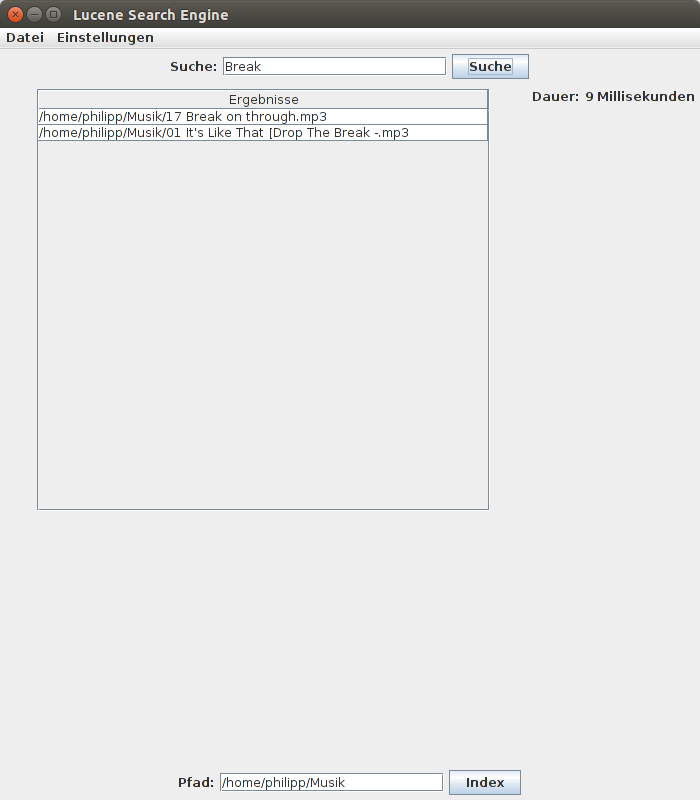
\includegraphics[width=7cm]{img/Lucene_Search_Engine_2.png}
\caption{Beispiel gesuchter Begriff\protect\footnotemark}
\end{figure}
\footnotetext{Quelle: Screenshot}
\subsection*{Der Indexer}
In diesem Teil möchte ich kurz auf die Klasse Index eingehen, welche nach den MP3-Dateien sucht und die Informationen aus den ID3-Tags zieht. 
\end{document}